\chapter{Análisis de experiencias electorales}
\label{Elecciones}

Toda persona involucrada en el proceso de votación (ciudadanos, partidos políticos, gobierno, entre otros) debe confiar en el sistema electoral para considerarlo exitoso.

\begin{comment}
Un sistema de votación exitoso debe cumplir el principal objetivo que es construir la confianza de toda persona involucrada en el proceso: ciudadanos, partidos políticos, gobierno, entre otros. Como posibles alternativas al sistema electoral tradicional, planteadas a nivel mundial, ha sido aplicar distintas técnicas para automatizar parte del proceso de votación. 
\end{comment}
Experiencias de implementación de voto electrónico obtuvieron diferentes niveles de aceptación y en algunos casos, luego de unos cuantos intentos, volvieron al sistema electoral tradicional.
En este capítulo se analizan elecciones con ejemplos de técnicas que computarizaron parte del proceso electoral. Se inicia el análisis en elecciones internacionales, luego con elecciones provinciales, y se finaliza con una encuesta sobre la opinión pública del voto electrónico implementado en Neuquén Capital.

\section{Elecciones Internacionales}
%\agregar{Descripción de la seccion - HECHO}
A continuación se eligieron algunos países que implementaron tecnología dentro del proceso de votación. Además se describen brevemente las consecuencias obtenidas y la decisión de cada gobierno en continuar o no con su implementación.

\subsection{Estados Unidos}

En un comienzo, en los años 50 y 60 se utilizaron boletas de tarjetas perforadas, técnica descripta en la Sección \ref{ClasificacionVotoElectronico} implementando el reconocimiento óptico de boletas. Este mecanismo generó mayores problemas al momento del escrutinio como por ejemplo:
\begin{itemize}
    \item abolladuras en el papel,
    \item se consideraban válidas las marcas sólo si todos los presentes estaban de acuerdo,
    \item se consideraban votos inválidos cuando las papeletas eran marcadas con pluma o perforadas más de una vez o perforadas de forma ambigua (por ejemplo, en la línea entre dos partidos) o sin perforación.
\end{itemize}

Como solución a los problemas evidentes de los sistemas de tarjetas perforadas, comienza el uso de los dispositivos de registro electrónico directo de votos (DRE). El uso de dispositivos de votación en EEUU cobró especial relevancia a partir del año 2000, luego de que las elecciones presidenciales en donde un gran número de votos no fueron registrados apropiadamente. Existieron debates sobre los dispositivos utilizados, y hubo causas judiciales en muchos estados respecto a su uso. Por ejemplo, en el estado de Pensilvania se produjeron varios problemas en el equipo de votación electrónica utilizados en Noviembre del 2019, generando suficiente desconfianza en el sistema de votación para las elecciones del 2020. Otro caso es el ocurrido en Nueva Jersey en el que los resultados fueron inmediatos pero el total de votos emitidos no coincidía con la suma de los votos emitidos por partido \cite{eleccionesEEUU}.

Como consecuencia a estas experiencias, en 2002 se aprueba la ley federal Help America Vote Act., que establece un organismo de control denominado Election Assistance Commission (EAC)\footnote{https://www.eac.gov/about\_the\_eac/help\_america\_vote\_act.aspx}. El EAC conforma un comité técnico para delinear recomendaciones y guías para los sistemas de votación, en aspectos de seguridad, testing de usabilidad y establecimiento de estándares y método de prueba para sistemas de votación electrónica. En 2007, la EAC comenzó el proceso de certificación de equipamiento de voto electrónico. Además esta comisión lleva registro de distintos problemas reportados sobre los dispositivos que se usan en la actualidad (Voting System Reports Collecction, 2017) \cite{problemasReportados}.

\subsection{Irlanda}

La primera propuesta de voto electrónico en Irlanda se realizó en 1998 y en el 2000 se introdujo la legislación que permitió el voto electrónico, utilizando dispositivos DRE. Para el 2002, se hicieron las primeras pruebas piloto con el objetivo de extenderlo al resto del país. Luego de unos meses, se filtra un informe confidencial del Ministerio del Interior irlandés a la prensa, allí se aseguraba que la integridad del proceso electoral no estaba garantizada. Entre otras fallas, el memorando interno que tomó estado público destacaba la posibilidad de que un software malicioso sencillo de programar pudiera generar una pantalla falsa en la máquina para hacer votar incorrectamente al elector. A pesar de esto, el gobierno irlandés avanzó con el plan de implementación para las elecciones locales y europeas de 2004. Se creó la Comisión Independiente de Votación y Escrutinio Electrónico para que examinara el sistema propuesto. La comisión emitió un informe \cite{informeIrlanda} en el que sostuvo que puede recomendar la utilización del sistema de voto electrónico pero no podía garantizar la seguridad del voto y la rigurosidad del escrutinio. El gobierno no dio marcha atrás con el sistema pero lo puso en suspenso. La inversión que hizo Irlanda en el sistema fue uno de los argumentos principales de las autoridades para no descartar el sistema. Como resultado se registró 52 millones de libras iniciales que se le pagaron a Nedap (Nederlandsche Apparatenfabriek)\footnote{https://nedap.com/}, y se agregaban los costos de mantenimiento y de actualización del sistema (calculando en 700.000 euros anuales y 20.000.000 por única vez) \cite{libroVoto}.

Finalmente, el 23 de abril de 2009 el entonces ministro anunció que quedaba descartado el sistema de voto electrónico, en base al alto costo de mantenimiento y actualización, sumado a la insatisfacción y sospechas que generó entre los electores. En 2019 se realizó una encuesta al público sobre el uso de elecciones electrónicas consiguiendo un 50\% de aceptación \cite{eleccionesIrlanda}.
\subsection{Holanda}
%\cambiar{ La batalla contra el voto electrónico en Holanda fue dada por un grupo de activistas informáticos denominado}
En el 2008 (un año antes que el caso irlandés) el gobierno de Holanda había tomado la misma decisión, abandonar el sistema de voto electrónico que había comprado a una empresa local, Nedap, utilizándose las mismas máquinas que en Irlanda. La batalla contra el voto electrónico en Holanda fue dada por un grupo de activistas informáticos denominado "We don't trust voting computers"\footnote{https://wijvertrouwenstemcomputersniet.nl/Wij\_vertrouwen\_stemcomputers\_niet}. Este grupo además de presentaciones judiciales, realizaron una demostración pública en un programa de televisión de las múltiples formas en las que se podía acceder y tomar el control de las máquinas Nedap sin demasiado esfuerzo. En menos de cinco minutos, lograron correr su propio software en una máquina de la empresa y repartir votos de acuerdo a sus preferencias, engañando al elector que utilizaba la máquina. Hasta el día de hoy, Holanda mantiene el sistema de voto por medio de boleta de papel \cite{netherlands}.

%\agregar{citar fuente sumado  artículos científicos por scholar por ejemplo https://ieeexplore.ieee.org/abstract/document/7001135 - HECHO}
\subsection{Estonia}
En las elecciones municipales del 2005, Estonia se convirtió en el primer país del mundo en probar el voto por Internet, descripta en la Seccion \ref{ClasificacionVotoElectronico} implementando el Sistema de votación a distancia. El sistema permite optativamente votar por Internet desde un lugar remoto, la identificación se hace a través del documento nacional de identidad que es una tarjeta inteligente. El voto por Internet es previo al día de la votación dejando al elector modificar su voto las veces que desee, tomándose como válido el último voto. En 2005, casi el 2\% utilizó el mecanismo de voto por Internet y fue creciendo hasta llegar al 30\% de la población en 2015. Las pocas garantías que ofrece sobre el carácter secreto del voto es una de las principales críticas que recibe este sistema. Los expertos consideraron que se debía suspender la aplicación de esta forma de votación, pero las quejas fueron rechazadas por el Comité de Voto por Internet del país y, en 2015, Estonia celebró sus elecciones con el sistema de voto por Internet \cite{vassil2016diffusion}.

%\agregar{citar fuente sumado  artículos científicos scholar - HECHO}

\subsection{Alemania}
A partir de 1998 Alemania comenzó a utilizar dispositivos electrónicos de voto DRE, desarrolladas por la empresa Nedap al igual que en Holanda. Comenzando con pruebas pilotos en Colonia y sucesivamente adoptados en distintas ciudades, y generalmente bien aceptadas por la ciudadanía, hasta 2005. En ese año, un par de ciudadanos presentaron una causa ante la Corte Constitucional Alemana, alegando que el uso de máquinas de votación electrónica es inconstitucional y que, dado que son vulnerables, los resultados de las presidenciales de 2005 no son confiables. Un fallo de esta corte dictaminó que el uso de las máquinas Nedap es inconstitucional, aunque no prohíbe el uso de cualquier dispositivo electrónico, sino que requiere que los mismos sean transparentes. Hoy Alemania usa la boleta única en papel \cite{volkamer2010electronic}.

%\agregar{citar fuente sumado  artículos científicos scholar - HECHO %? \url{http://www.brunazo.eng.br/voto-e/textos/CIPPEC-Brunazo.htm}
%\url{http://www2.congreso.gob.pe/sicr/cendocbib/con2_uibd.nsf/1B5274E790C782A1052577BB0075538C/\$FILE/El\_Voto\_Electr\%C3\%B3nico_en_Brasil.pdf}}
\subsection{Brasil}
En 2002 implementó una elección a escala nacional utilizando unos 406.000 dispositivos electrónicos DRE en la cual más de 100 millones de votantes emitieron su sufragio. Los reportes de testing de seguridad públicos en 2012 muestran que existen problemas técnicos severos en los dispositivos utilizados. Entre los problemas más relevantes se señalan la inadecuada protección del secreto del voto, el uso inapropiado de encriptación y algoritmos de criptografía obsoletos, modelos de ataques inadecuados centrados en atacantes externos cuando los ataques internos presentan un riesgo mucho mayor, adopción de un proceso de desarrollo de software defectuoso y verificación de integridad insuficiente \cite{brunazo2005voto}.

\section{Experiencias en Argentina}

Además de las experiencias de implementación de voto electrónico en distintos países con variadas técnicas, tenemos ejemplos a nivel nacional en Elecciones Municipales, Provinciales y Nacionales. Estas experiencias tuvieron diferentes niveles de aceptación, metodologías y distintas fases del proceso de votación que involucraron tecnología. En las siguientes subsecciones se describen ejemplos de experiencias en Argentina.

\subsection{Elección Municipal de Las Grutas}
El 16 de diciembre de 2007 se utilizaron 4 urnas electrónicas de la firma Altec\footnote{https://www.altec.com.ar/} (Rio Negro) en la localidad de Las Grutas (Argentina). El proceso electoral se realizó con una tarjeta magnética que se le otorga al elector al momento del sufragio, y en la que se graban las opciones seleccionadas. La tarjeta luego se ingresa a la tradicional urna electoral junto a la boleta electrónica impresa por el dispositivo. Estas máquinas además valida al votante, esto generó momentos de tensión debido a que la urna algunas veces no habilitaba al votante siendo que en el padrón en papel figuraba. Otro de los problemas fueron máquinas que se trababan y al trabarse el papel utilizado dejaba en evidencia la elección del votante. La utilización de estas urnas electrónicas se implementó a pesar que el 10\% de los habitantes del lugar elevaran al superior tribunal de justicia la no obligatoriedad de este sistema \cite{eleccionesLasGrutas}.
\subsection{Elecciones Provinciales de Neuquén}

El 10 de Marzo de 2019, Neuquén realizó la elección para gobernador y vicegobernador por medio del sistema de Boleta Única Electrónica (BUE), y con el sistema tradicional en papel en mesas con menor concurrencia. Previo a esta elección existió una etapa de fiscalización para verificar y auditar el sistema utilizado, se armó un resumen de esta experiencia expuesta en el Anexo \ref{fiscalizacionNeuquen}, además se publicó un artículo en JAIIO \cite{articuloGukenaFiscalizacion}. Las BUE son boletas que contienen un chip electrónico RFID (Radio Frequency Identification)\cite{rfc} donde se almacena el voto, además de imprimirse al dorso en letra legible.
La Figura \ref{fig:maquinasBUE} muestra una máquina con una BUE de ejemplo, estas máquinas son manipuladas directamente por el votante, imprimiendo su votación sobre una BUE para luego ser utilizada para el escrutinio de cada mesa. El proceso de votación para estas elecciones se conformó de la siguiente manera:
\begin{figure}
\begin{center}
  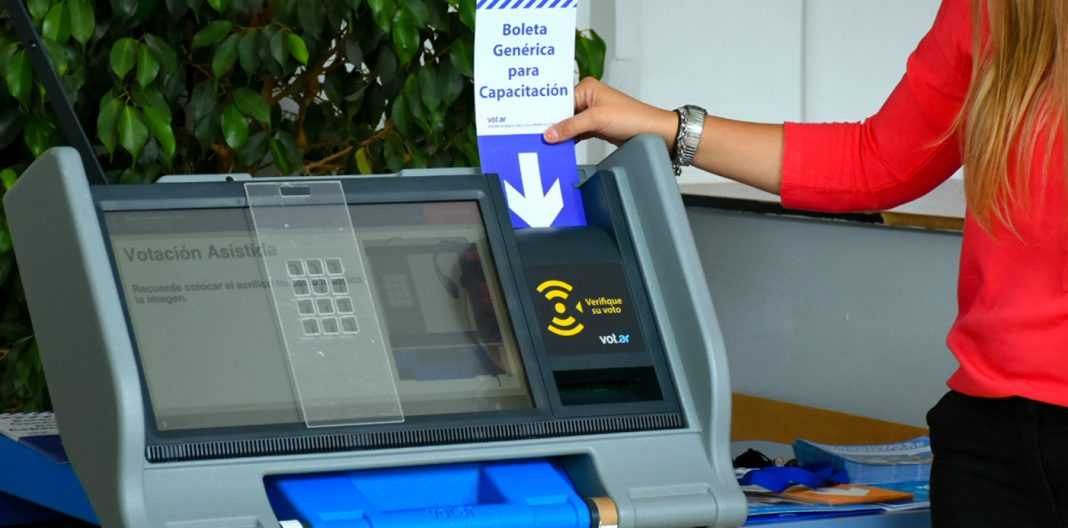
\includegraphics[scale=0.4]{img/Maquina_BUE.jpg}
  \caption{Máquina utilizada en las elecciones de Neuquén}
  \label{fig:maquinasBUE}
\end{center}
\end{figure}
\begin{itemize}
    \item Votación utilizando la máquina electrónica.
    \item Conteo utilizando la maquina electrónica y las boletas electrónicas.
    \item Envío de datos desde las escuelas con la máquina electrónica utilizando el certificado generado de cada escrutinio de la mesa.
    \item Resultados provisorios.
\end{itemize}

Sobre estas elecciones se obtuvieron los siguientes datos\footnote{\url{http://200.70.33.130/images2/Electoral/CP_10-03-2019/Info\_general/datos\_generales\_de\_la\_eleccion.pdf}}:
\begin{itemize}
    \item 493.760 neuquinos estuvieron habilitados para votar, de los cuales se contabilizó una participación del 78.44\%.
    \item 1.504 mesas distribuidas en 283 escuelas, de las cuales 191 trabajaron con el sistema BUE, 86 con el sistema tradicional de papel y 6 escuelas tuvieron ambos sistemas.
\end{itemize}

Con respecto a la velocidad de cómputo y publicación, en la Figura \ref{graf:porcentajeNeuquen} se muestra la información del porcentaje de mesas cargadas incrementalmente en periodos de 10 minutos desde el cierre del acto electoral. Podemos notar que existen tres periodos durante el escrutinio. Durante las primeras dos horas no se registran mesas en el sistema ya que cada una está siendo escrutada. Luego se percibe una carga masiva simultánea de más del 50\% de las mesas escrutadas. Por último, podemos ver una curva lenta durante la carga hasta completar la totalidad de las mesas.

En la Figura \ref{graf:velocidadNeuquen} se observa la velocidad de la carga (cantidad de mesas cargadas por minuto) distribuido en periodos de 10 minutos desde el cierre del acto electoral. Al igual que la figura anterior, podemos notar un pico luego de dos horas del comienzo del escrutinio, siendo el momento de mayor carga de información simultánea de las mesas escrutadas. Luego de este pico la velocidad en la carga es más relajada hasta completar la totalidad del escrutinio.

Con el objetivo de obtener estos datos utilizamos la técnica de Web Data Scraping, esta técnica se basa en un script de extracción y combinación de contenido alojado en la Web de manera sistemática. Se extraen los datos de interés y se lo estructura como se lo desee \cite{glez2014web}.
Luego de finalizado el escrutinio se ejecutó un pequeño script que extrae y estructura la información obtenida a través de una API, provista por la provincia de Neuquén. 

\begin{figure}[h!]
  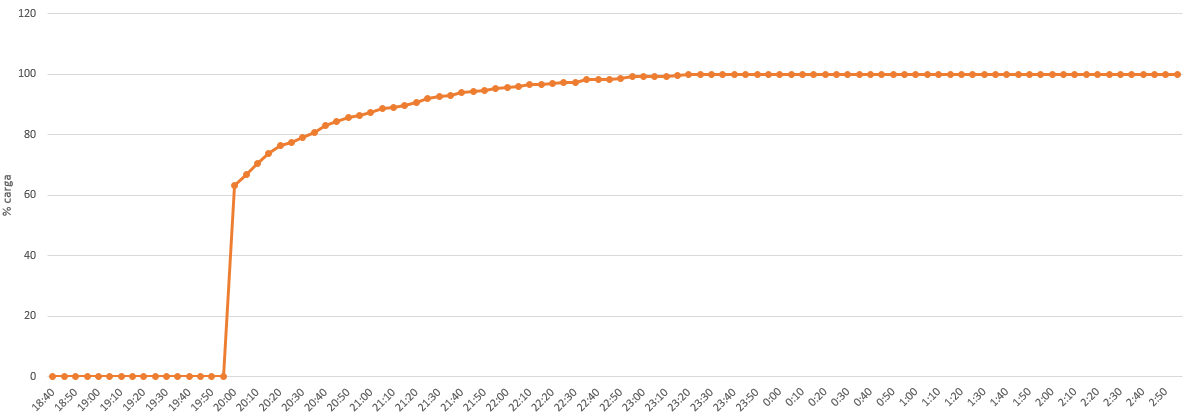
\includegraphics[width=1\textwidth]{img/fOI0sHj9ac.png}
  \caption{Porcentaje de mesas cargadas - Neuquén (2019)}
  \label{graf:porcentajeNeuquen}
\end{figure}

\begin{figure}[h!]
  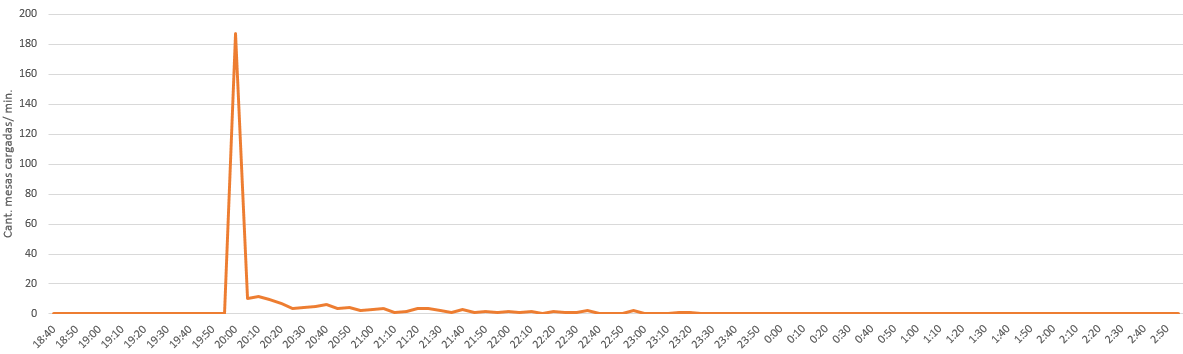
\includegraphics[width=1\textwidth]{img/QOsSnICbyL.png}
  \caption{Velocidad en carga de mesas - Neuquén (2019)}
  \label{graf:velocidadNeuquen}
\end{figure}


\subsection{Elecciones Provinciales de Rio Negro}

El 7 de Abril de 2019, Río Negro realizó la elección para gobernador y vicegobernador por medio del sistema tradicional de votación en papel. Cada votante contenía en su sobre su lista o listas elegida/s en papel y, el escrutinio se realiza manualmente enviándose los datos desde cada escuela por medio de telegramas. En estas elecciones se utilizó tecnología sólo en la fase de publicación. El proceso de votación para esta elección se conformó con los siguientes elementos:
\begin{itemize}
    \item 7 listas candidatas que el elector debe elegir.
    \item 546.067 electores habilitados, esto quiere decir que se prepararon 546.000 sobres aproximadamente, uno por cada elector.
    \item 1646 mesas, esto implica la misma cantidad de urnas.
\end{itemize}
Teniendo estos datos se puede concluir que sólo para elecciones de gobernador y vice se utilizaron aprox. 3.822.000 papeles, 7 listas preparadas para 546.000 electores. A través de la técnica Web Scraping se obtuvo la información necesaria para su análisis.

En la Figura \ref{graf:porcentajeRioNegro} se dispuso la información del porcentaje de mesas cargadas incrementalmente en periodos de 10 minutos desde el cierre del acto electoral. Durante las primeras dos horas no se registran mesas en el sistema ya que cada una está siendo escrutada simultáneamente. Luego se observa una curva constante hasta completar la totalidad de las mesas.

En la Figura \ref{graf:velocidadRioNegro} se dispuso la velocidad de la carga (cantidad de mesas cargadas por minuto) distribuido en periodos de 10 minutos desde el cierre del acto electoral. Como en la figura anterior durante las primeras dos horas del escrutinio no se registra movimiento de información. Luego se observa una carga uniforme hasta completar la totalidad de las mesas. 

\begin{figure}[h!]
  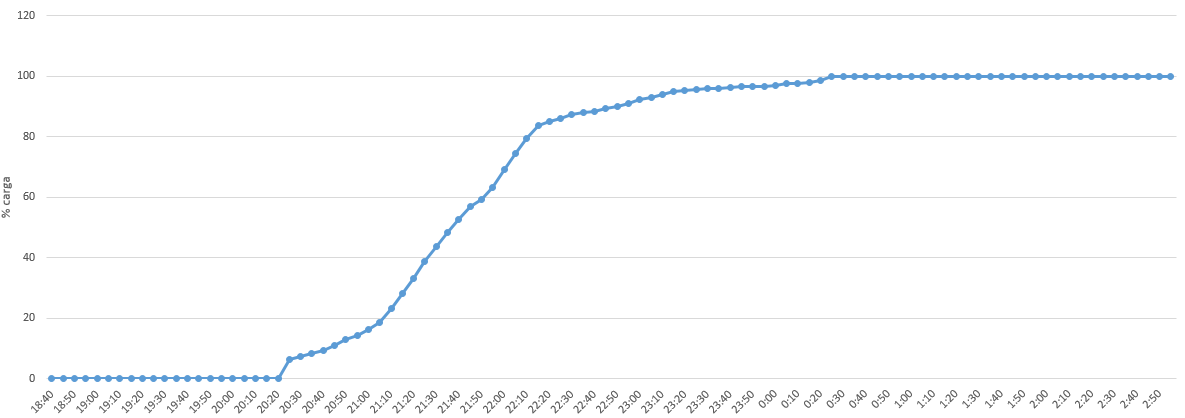
\includegraphics[width=1\textwidth]{img/sAveHlGEkX.png}
  \caption{Porcentaje de mesas cargadas - Rio Negro (2019)}
  \label{graf:porcentajeRioNegro}
\end{figure}

\begin{figure}[h!]
  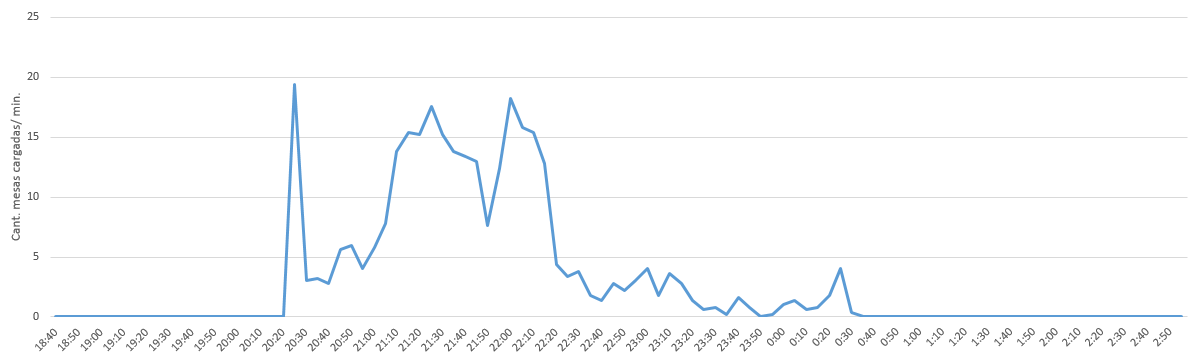
\includegraphics[width=1\textwidth]{img/8w25IVQD5U.png}
  \caption{Velocidad en carga de mesas - Rio Negro (2019)}
  \label{graf:velocidadRioNegro}
\end{figure}

\subsection{Elecciones Provinciales de Córdoba}

El 12 de Mayo de 2019, Córdoba realizó la elección para gobernador, legisladores,  candidatos a ocupar el tribunal de cuentas provincial, y en algunas localidades se renovaron autoridades municipales, por medio del sistema de Boleta Única de Sufragio (BUS) \cite{cortiboleta}, en Córdoba se tomó la denominación BUS para la Boleta Única en Papel. Este método consta de una única boleta impresa con todos los cargos y candidatos 
%\cambiar{cv sobre la cual} 
sobre la cual el votante indica su elección dentro de esta boleta, luego 
%\cambiar{cv se la ingresa} 
se la ingresa en la urna. En las columnas se organizan cada uno de los cargos y en las filas se listan los espacios políticos como se puede ver en la Figura \ref{graf:BUSCordoba}.
\begin{figure}[h!]
  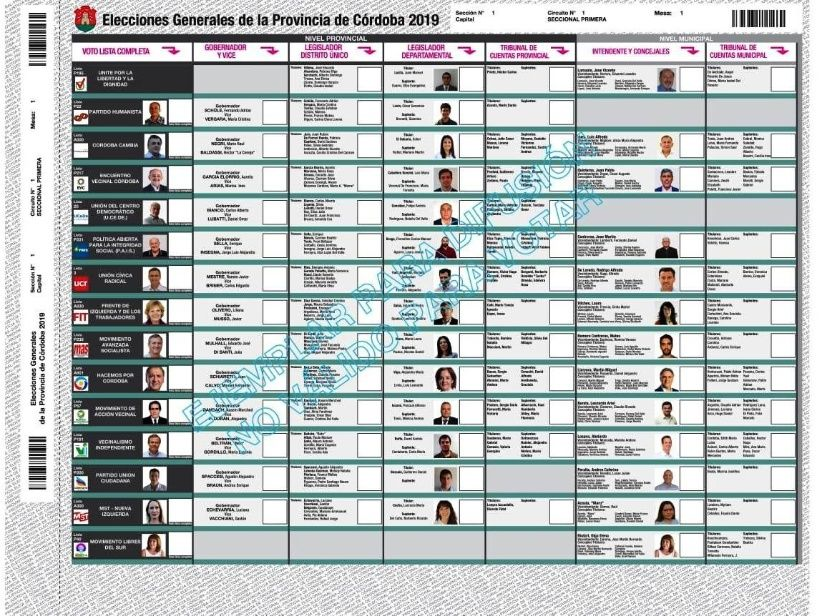
\includegraphics[width=1\textwidth]{img/boletaunica-cordoba.jpg}
  \caption{Ejemplo de la Boleta Única de Sufragio (BUS)}
  \label{graf:BUSCordoba}
\end{figure}
En estas elecciones se incluyó tecnología en la fase de Publicación de resultados, el escrutinio es manual enviándose los datos de cada escuela por medio de telegramas. El proceso de votación para esta elección se conformó con los siguientes elementos: 
\begin{itemize}
    \item 13 listas candidatas para gobernador que el elector debe elegir.
    \item 2.889.973 electores habilitados, esto quiere decir que se prepararon 2.889.000 boletas aproximadamente, uno por cada elector.
    \item 8654 mesas.
    \item 320 millones de pesos costó este sistema. 
\end{itemize}
%\cambiar{3.000.000 de boletas un poco más por las dudas. - HECHO}
Debido a que se utiliza una boleta por elector, se puede concluir que sólo para elecciones de gobernador y vice se utilizaron cerca de 3.000.000 boletas en papel. De igual manera que en las elecciones de Neuquén y Río Negro, se obtuvieron los datos de las elecciones utilizando la técnica de Web Data Scraping, obteniendo una evolución de carga de mesas representado en la Figura \ref{graf:porcentajeCordoba} y su velocidad de carga en la Figura \ref{graf:velocidadCordoba}. Como se puede ver, los datos fueron agrupados en fracciones de 10 minutos durante todo el proceso de escrutinio. Entre las 20:00 hrs y 00:00 hrs se observa una velocidad de carga de 15 a 55 mesas por minuto, con respecto al porcentaje de carga se ve un crecimiento constante hasta completar la totalidad de las mesas.

\begin{figure}[h!]
  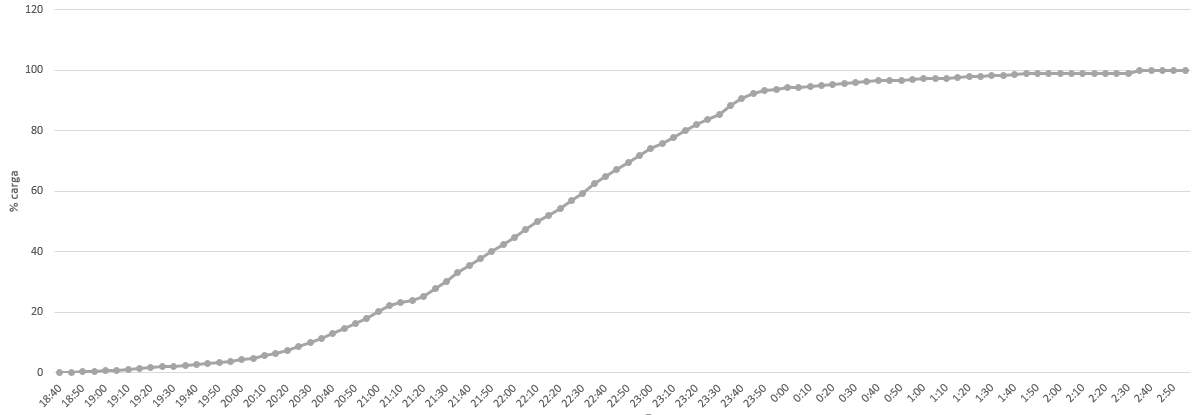
\includegraphics[width=1\textwidth]{img/E4YqKc5Tcu.png}
  \caption{Porcentaje de mesas cargadas - Córdoba (2019)}
  \label{graf:porcentajeCordoba}
\end{figure}

\begin{figure}[h!]
  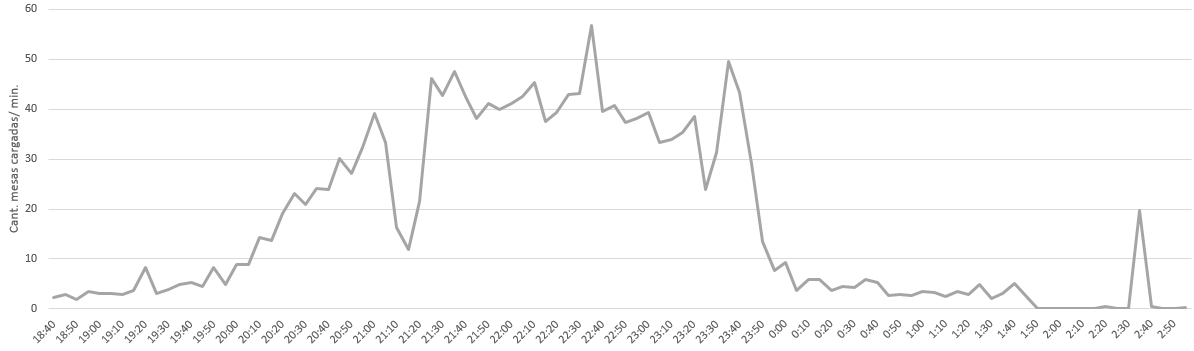
\includegraphics[width=1\textwidth]{img/9rEiyqeSFw.png}
  \caption{Velocidad en carga de mesas - Córdoba (2019)}
  \label{graf:velocidadCordoba}
\end{figure}

\subsection{Sistema Escrutinio Nacional}
En 2019 se utilizó el sistema llamado SmartTally\footnote{https://www.smartmatic.com/es/elecciones/elecciones-manuales/smarttally/}, que consta en el envío de telegramas directo desde el establecimiento hacia los centros de cómputos de la Dirección Nacional Electoral (DINE), que depende del Ministerio del Interior de la Nación. El transporte y servicio de logística es llevado a cabo por el Correo Argentino. Cada establecimiento consta de una impresora multifunción, conexión a Internet y un equipo que permite la conexión y monitoreo del envío exitoso de los telegramas. \newline
Este sistema se usó para las elecciones las PASO (Primarias, Abiertas, Simultáneas y Obligatorias) el 11 de Agosto de 2019, y en las Elecciones Nacionales el 27 de Octubre de 2019.

Polémicas al usar este tipo de sistema:
\begin{itemize}
    \item Auditabilidad del Software: Se requirió que la empresa ponga a disponibilidad el software usado para su investigación, a modo de reconocer posibles fallas. Frente a este pedido el Gobierno notifica que no es posible ya que el software es alquilado y la empresa dueña se niega a entregar este producto \cite{auditabilidadSmartmatic}.
    \item Seguridad frente a ataques externos: Javier Smaldone presentó vulnerabilidades en el software de conversión de formato de los ``telegramas'' electorales poniendo en riesgo la integridad del proceso \cite{seguridadSmartmatic}.
    \item Transparencia: Debido a que este sistema consta de dos etapas en el proceso de escrutinio, existe cierta desconfianza entre los datos cargados por cada transmisión exponiendo los resultados provisorios y el resultado final luego de ser validado dentro de los 10 días como indica el código electoral. Este primer resultado podría generar datos ganadores que luego no son así en el resultado final \cite{rnEscrutinioProvisorio}.
\end{itemize}



\section{Análisis de la utilización de Tecnología en Elecciones}

El año 2019 fue un año ideal para el análisis de sistemas electoral nacionales, se realizaron múltiples elecciones a nivel municipal, provincial y nacional. Además de las magnitudes en cada elección se implementaron distintas técnicas en el proceso de elección. Esto permitió tomar experiencias y realizar una comparación de velocidad de publicación de resultados. A continuación de describe un análisis de las elecciones provinciales en Neuquén, Rio Negro y Córdoba, cuyas elecciones utilizaron diferentes técnicas. Con respecto a la ciudad de Neuquén Capital se realizó una encuesta del nivel de aceptación, confianza y conocimiento del sistema BUE utilizado en tres ocasiones anteriores a estas elecciones del 2019, por lo tanto, existía un aprendizaje de la población.

\subsection{Análisis comparativo en Elecciones Provinciales de Neuquén, Córdoba y Río Negro}
\label{analisisComparativoProvincial}

A través de resultados almacenados en \textit{datosoficiales.com} se consiguieron los datos de cada elección  en 2019 detallada en las secciones anteriores de Neuquén, Río Negro y Córdoba.   \newline
En estas tres experiencias, las provincias contrataron a la empresa MSA\footnote{MSA \url{https://www.msa.com.ar/}} aplicando tecnología en diferentes fases, como se detalló anteriormente, y logrando los resultados como se muestra en la Tabla \ref{tab:comparativa}.
\begin{table}[]
    \centering
    \begin{tabular}{|c|c|c|c|}
        \hline
         Provincia & Neuquén& Río Negro & Córdoba   \\
         \hline
         Técnica utilizada& BUE & Tradicional & BUS \\
         \hline
         Electores& 493.760 & 546.067 & 2.889.973 \\
         \hline
         Mesas& 1.504 & 1.646 & 8.654\\
         \hline
         Tecnología aplicada a& Emisión de Voto &Comunicación & Comunicación \\
         & Generación de Documentos & de Resultados &  de Resultados\\
         & Comunicación de Resultados & & \\
         \hline
         *Computado el 80\% & 20:30 & 21:10 & 23:20\\
         \hline
    \end{tabular}
    \caption{Comparativa de diferentes métodos utilizados en elecciones provinciales de 2019}
    \label{tab:comparativa}
\end{table}


En la Figura \ref{fig:velocidad} se puede observar la velocidad comparativa de la carga de datos en cada provincia, y en la Figura \ref{fig:acumulado} se representa el porcentaje acumulado durante el periodo de escrutinio. En estos gráficos, la linea naranja representaría las elecciones utilizando BUE, la linea gris las elecciones utilizando BUS y la linea azul es el resultado de las elecciones tradicionales con boletas partidarias de papel. \newline
A primera impresión se puede observar la notable velocidad de carga en la provincia de Neuquén en los primeros minutos de las 20:00 hs., satisfaciendo el objetivo de rapidez de las máquinas BUE. Sin embargo, se reduce su velocidad hasta completar la totalidad de las mesas. Por otro lado, la provincia de Córdoba, por medio de la BUS logra una velocidad constante de carga hasta completar la totalidad de las mesas. Como se puede observar en la Figura \ref{fig:acumulado} la completitud de las mesas escrutadas se logra con poca diferencia de horas, dando a notar que aplicando tecnología en cualquier etapa del escrutinio no genera un impacto notable en la velocidad de los resultados. 
Al igual que para las elecciones sobre estas provincias, se intentó aplicar la técnica de Web Data Scraping y evaluar la velocidad de carga en las elecciones nacionales PASO y Generales de 2019. Sin embargo, no se logró obtener datos útiles para nuestro propósito ya que estos datos no contenían fechas y horas de publicación de cada mesa. Igualmente, en las Elecciones Generales 2019 a las 21:00 hrs. se logró publicar un 80\% del total de mesas, lo que muestra una técnica con muy buenos tiempos de velocidad de publicación de resultados.

\newline

\begin{figure}[h!]
  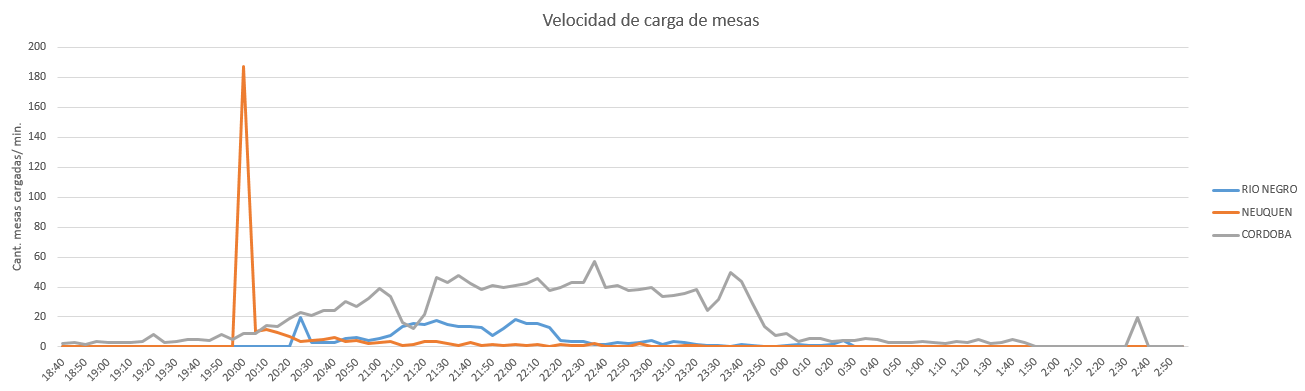
\includegraphics[width=\textwidth]{img/grafico_velocidad_carga.png}
  \caption{Velocidad de Cargas de mesas}
  \label{fig:velocidad}
\end{figure}
\begin{figure}[h!]
  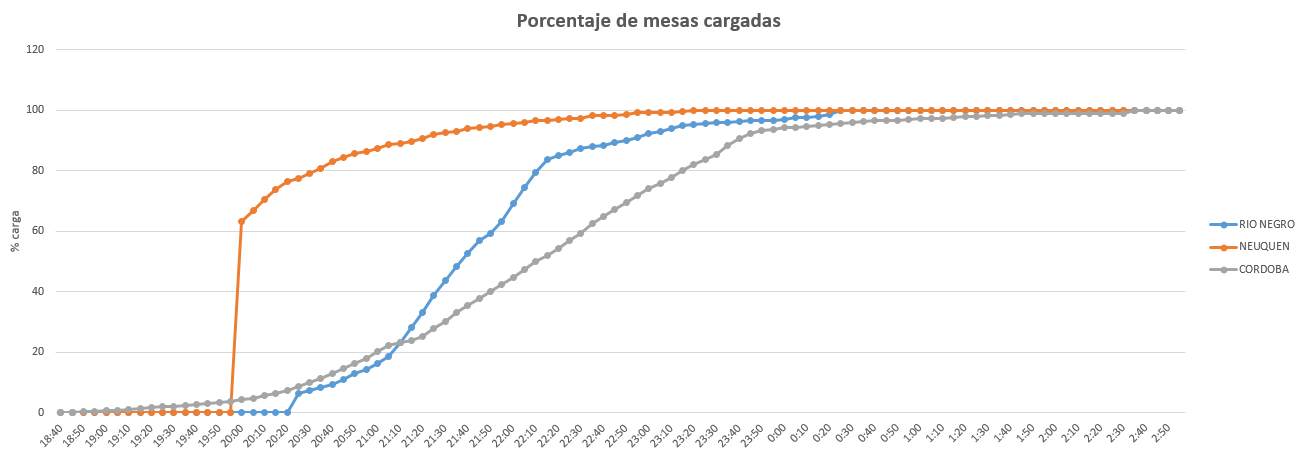
\includegraphics[width=\textwidth]{img/carga_mesas.png}
  \caption{Porcentaje de mesas cargadas}
  \label{fig:acumulado}
\end{figure}

%Otra elección que logró implementar un sistema electoral tradicional sin intervención tecnológica utilizando la BUS fue en San Carlos de Bariloche, el 1 de Septiembre del 2019\footnote{Noticia: https://www.anbariloche.com.ar/noticias/2019/08/24/70978-elecciones-municipales-como-se-vota-con-la-boleta-unica}. 
Una característica que puede generar inconvenientes de la BUS es el tamaño que puede conseguir, ya que tiene que contener todas las listas disponibles. Por ejemplo, en las elecciones de Córdoba se tiene un tamaño de 40 cm de alto por 47 cm de ancho como modelo general, este tamaño podría extenderse en municipios o dependiendo de la cantidad de partidos o alianzas que se presenten \cite{boletaUnicaTamanio}. \newline
Dentro del modelo de referencia, el sistema BUE consta de las fases de Emisión del voto y además esta boleta es utilizada para la fase posterior de Escrutinio de la mesa. Varios municipios utilizaron este sistema, a pesar del debate impulsado por varias instituciones en contra del uso de este método. Un inconveniente que puede albergar es la limitación en la pantalla. Una pantalla dispone de 18 lugares para ubicar a los candidatos. Con el uso de listas colectoras se llegaron a multiplicar las listas. La disposición de los candidatos en la pantalla de estas máquinas puede afectar la accesibilidad de los electores al reducirse el tamaño de cada cuadricula. Como ejemplo, en Plottier \cite{lmncolectoras} se dispusieron 29 candidatos a intendencia de la ciudad y 26 en Neuquén. 
\subsection{Análisis sobre la opinión pública sobre las elecciones en Neuquén Capital}
\label{encuesta}

Como aporte a esta tesis el día 22 de Septiembre de 2019, durante las elecciones a intendente en Neuquén Capital, se realizó una encuesta con la intención de conocer la opinión de los votantes, con preguntas relacionadas a la interacción que tuvo cada votante con la máquina BUE al momento de registrar su voto. Esta actividad fue realizada junto con el Lic. Pablo Kogan a una distancia permitida de la escuela elegida, por Código Electoral no se permite ninguna encuesta durante el acto electoral en un radio de 100 metros del establecimiento de votación. La encuesta consistió de una mínima cantidad de preguntas y que sean muy sencillas de entender, cada votante que aceptaba ser encuestada no tardaba más de 5 minutos en responder.

Al ser un municipio con 4 elecciones utilizando el sistema BUE, es una buena muestra de votantes con experiencia. Esta actividad involucró votantes de cuatro escuelas repartidas en puntos importantes de la ciudad. Las escuelas elegidas fueron Esc. nº201 (Barrio Centro), nº 40 (Barrio San Lorenzo), nº 20 (Barrio Don Bosco) y nº 103 (Barrio Confluencia) logrando encuestar 145 personas en total. \newline
El objetivo de esta encuesta fue conocer el nivel de aprendizaje de los votantes sobre este nuevo sistema y en respuesta a su uso, cuánta confianza y facilidad les resulta este medio de votación. A cada votante se le hacían cinco preguntas con opciones de respuesta, estas opciones pueden ser Si, No o un intermedio que denominamos Maso.
\begin{itemize}
    \item P1. ¿La persona encuestada votó? SI/NO
    \item P2. ¿La persona encuestada leyó su boleta impresa? SI/NO
    \item P3. ¿La persona encuestada verificó su boleta utilizando el lector de chip RFID? SI/NO
    \item P4. ¿A la persona encuestada le resulta simple votar con la boleta BUE? SI/NO/MASO
    \item P5. ¿La persona encuestada confía en el sistema de votación utilizada? SI/NO/MASO
\end{itemize}

Se decidió subdividir las muestras por edad generacional, dado a que la edad no formó parte de la encuesta se anotaba este dato en base a nuestro criterio. Por lo tanto, se encuadra cada votante dentro de las categorías
\begin{itemize}
    \item Generación Z: Personas nacidas a partir del 2000, representado en la tabla como menores a 25 años aprox.
    \item Generación Y: Personas nacidas entre 1980-1999, representado en la tabla con edades entre 25 y 39 años aprox.
    \item Generación X: Personas nacidas entre 1965-1979, representado en la tabla con edades entre 39 y 55 años aprox.
    \item Generación BG: Personas nacidas entre 1946-1964, representado en la tabla con edades mayores a 55 años aprox.
\end{itemize}
A partir de esta actividad se obtuvieron los datos de la Tabla \ref{tab:encuesta} donde se contabiliza la cantidad de personas que respondieron a cada opción para cada pregunta.

\begin{table}[h!]
\caption{Resultado sobre los encuestados}
\begin{center}
\resizebox{\textwidth}{!}{
\begin{tabular}{ |c|c||c|c|c||c|c|c||c|c|c||c|c|c|c| } 
 \hline
 \multirow{2}{4em}{Pregunta} & \multirow{2}{3em}{Generación} & \multicolumn{3}{|c||}{Escuela nº201} & \multicolumn{3}{|c||}{Escuela nº40} & \multicolumn{3}{|c||}{Escuela nº20} & \multicolumn{3}{|c|}{Escuela nº103} & \multirow{2}{3em}{Total}\\
  & &SI & MASO & NO & SI & MASO & NO & SI & MASO & NO & SI & MASO & NO & \\ 
 \hline
 \multirow{4}{3em}{P1. ¿Votó?} & Z < 25 & 2 & \cellcolor{gray} & & 7 & \cellcolor{gray} & & 4 &\cellcolor{gray} & & 5 &\cellcolor{gray} & & 18 \\ 
 & 25 <= Y < 39 & 8 &\cellcolor{gray} & & 12 &\cellcolor{gray} & & 12 &\cellcolor{gray} & & 4 &\cellcolor{gray} & & 36\\ 
 & 39 <= X < 55 & 15 &\cellcolor{gray} & & 12 &\cellcolor{gray} & & 13 &\cellcolor{gray} & & 23 &\cellcolor{gray} & & 63 \\
 & 55 <= BG & 12 &\cellcolor{gray} & & 5 &\cellcolor{gray} & & 7 &\cellcolor{gray} & & 4 &\cellcolor{gray} & & 28\\ 
 \hline \hline
 \multirow{4}{3em}{P2. ¿Leyó?} & Z < 25 & 1 &\cellcolor{gray} & 1 & 6 &\cellcolor{gray} & 1 & 4 &\cellcolor{gray} & & 5 &\cellcolor{gray} & & 18\\ 
 & 25 <= Y < 39 & 8 &\cellcolor{gray} & & 11 &\cellcolor{gray} & 1 & 11 &\cellcolor{gray} & 1 & 4 &\cellcolor{gray} & & 36\\ 
 & 39 <= X < 55 & 15 &\cellcolor{gray} & & 9 &\cellcolor{gray} & 3 & 11 &\cellcolor{gray} & 2 & 20 &\cellcolor{gray} & 3 & 63 \\
 & 55 <= BG & 11 &\cellcolor{gray} & 1 & 3 &\cellcolor{gray} & 2 & 7 &\cellcolor{gray} & & 3 &\cellcolor{gray} & 1 & 28 \\ 
 \hline \hline
 \multirow{4}{3em}{P3. ¿Verificó?} & Z < 25 &  &\cellcolor{gray} & 2 & 6 &\cellcolor{gray} & 1 & 1 &\cellcolor{gray} & 3 & 4 &\cellcolor{gray} & 1 & 18 \\ 
 & 25 <= Y < 39 & 5 &\cellcolor{gray} & 3 & 4 &\cellcolor{gray} & 7 & 8 &\cellcolor{gray} & 4 & 3 &\cellcolor{gray} & 1 & 36\\ 
 & 39 <= X < 55 & 8 &\cellcolor{gray} & 7 & 7 &\cellcolor{gray} & 6 & 4 &\cellcolor{gray} & 9 & 14 &\cellcolor{gray} & 9 & 63 \\
 & 55 <= BG & 5 &\cellcolor{gray} & 7 & 4 &\cellcolor{gray} & 1 & 4 &\cellcolor{gray} & 3 & 3 &\cellcolor{gray} & 1 & 28\\ 
 \hline \hline
 \multirow{4}{3em}{P4. ¿Es simple?} & Z < 25 & 2 & & & 6 & 1 & & 4 & & & 5 & & & 18 \\ 
 & 25 <= Y < 39 & 8 & & & 11 & & & 11 & 1 & & 4 & & & 35 \\ 
 & 39 <= X < 55 & 14 & & 1 & 12 & 1 & & 11 & 1 & 1 & 21 & 2 & & 64 \\
 & 55 <= BG & 12 & & & 3 & & 2 & 6 & & 1 & 2 & & 2 & 28 \\ 
 \hline \hline
 \multirow{4}{3em}{P5. ¿Confía?} & Z < 25 & 2 & & & 3 & & 4 & 1 & & 3 & 3 & 2 & & 18 \\ 
 & 25 <= Y < 39 & 4 & 3 & 1 & 1 & 4 & 6 & 6 & 1 & 5 & 1 & 1 & 2 & 33 \\ 
 & 39 <= X < 55 & 10 & 3 & 2 & 4 & 3 & 6 & 8 & 2 & 3 & 14 & 6 & 3 & 64\\
 & 55 <= BG & 10 & 2 & & & 1 & 4 & 3 & & 4 & 2 & & 2 & 28\\ 
 \hline \hline
\end{tabular}
}
\label{tab:encuesta}
\end{center}
\end{table}

Con los datos finales, se logra ver una gran cantidad de personas que leen sus boletas impresas pero no así con la lectura del chip integrado en la boleta, como se observa en la Figura \ref{graf:votantes}. A pesar de haber experimentado este sistema en distintas elecciones se descubrió que muchos de ellos no sabían la existencia del lector de chip, dato que no se esperaba. Como se puede ver en el gráfico cerca del 50\% desconocía esta verificación y no varía según la edad generacional.

\begin{figure}[h!]
  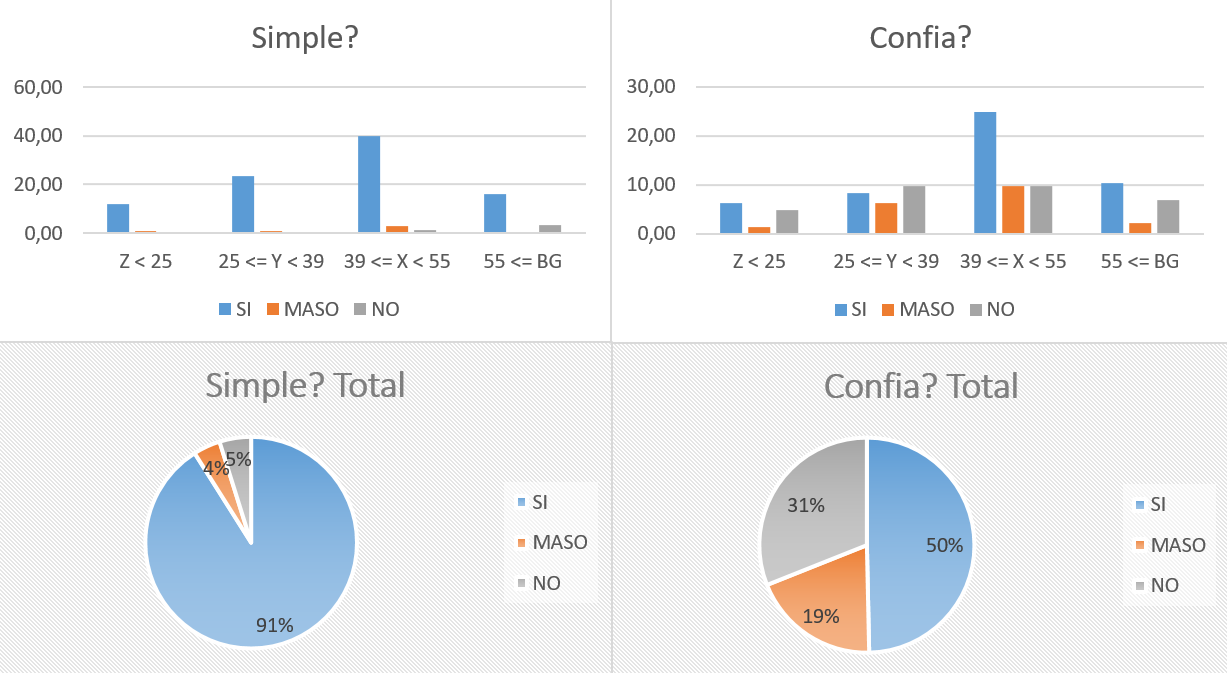
\includegraphics[width=\textwidth]{img/wJTgsdwuNh.png}
  \caption{Comparación entre los que leen y verifican su boleta electrónica}
  \label{graf:votantes}
\end{figure}

%\cambiar{Supone que la verificación de la boleta con chip era desconocida por el votante, y en realidad es una suposición ya que la podrían no haber querido corroborar.}
%\cambiar{En el diálogo con las personas que participaron de la encuesta, comentaron que no sabían que existía la posibilidad de verificar el voto.}

Otro dato curioso de estas opiniones es que casi la totalidad de las personas les resulta sencillo su uso, sin embargo, muy pocas de ellas les genera confianza. Como se puede ver en la Figura \ref{graf:votantesUsoConfia} la mitad de los encuestados les genera confianza o intentan confiar en este sistema. Sobre esta última característica destaca la variación de opiniones según la zona urbana encuestada, como se puede ver en la Tabla \ref{tab:encuesta}, en el área centro (Escuela nº201)  se concentra la cantidad de personas que confían en sistema BUE, seguido del área Confluencia (Escuela nº40). %\cambiar{Por otro lado las escuelas que se encuentran en zonas mas alejadas del centro no confían en este sistema. - HECHO}
Por otro lado las demás escuelas en zonas más alejadas del centro no logran confiar en este sistema. 

Otro dato que podemos observar por edad generacional, la generación X posee mayor confianza en el sistema BUE y son las personas que más leyeron el dato impreso en su boleta no así en la verificación, aunque fue la generación que más verificó, si analizamos solo ésta generación sólo la mitad de ellos validó el dato almacenado en el chip de la boleta.

\begin{figure}[h!]
  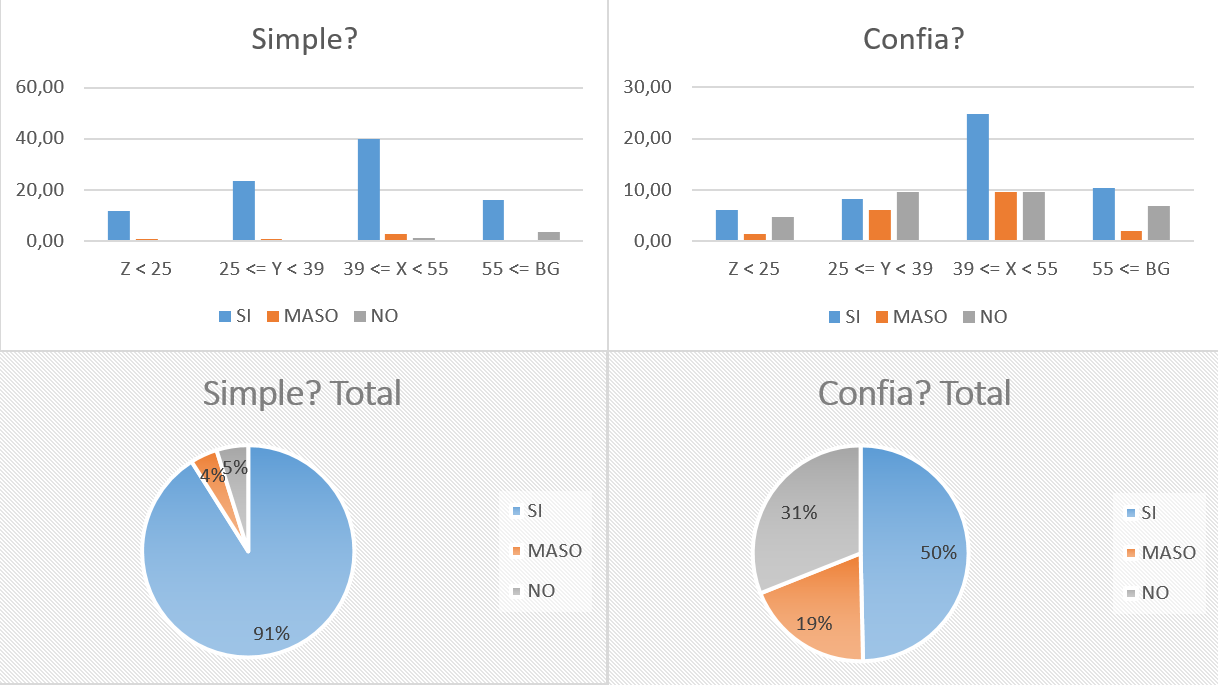
\includegraphics[width=\textwidth]{img/GGEjN1UUOE.png}
  \caption{Usabilidad vs. Confiabilidad}
  \label{graf:votantesUsoConfia}
\end{figure}

\section{Conclusión}

Luego de haber analizado en el Capítulo \ref{SistemaElectoral} las técnicas existentes para involucrar tecnología en el proceso electoral, pudimos ver en este capítulo varios intentos de implementación de ellas a distinta escala. Sin embargo, en estos intentos no se logró satisfacer el objetivo principal de un sistema electoral: la confianza de toda persona involucrada. Como pudimos ver, en varios países se ha intentado incluir tecnología en la primera fase de Emisión del Voto, consiguiendo un alto riesgo que luego es descubierto por distintas agrupaciones o entidades. Otro de los ejemplos es el resultado arrojado por la encuesta realizada en el municipio de Neuquén Capital, arrojando que el 50\% de la muestra no confía plenamente en el sistema BUE.

La principal justificación de incluir tecnología en la fase de Emisión del Voto es la mejora en la velocidad de carga y conseguir los datos finales en el menor tiempo. Sin embargo, como se pudo validar en los resultados obtenidos en las elecciones provinciales de Neuquén, Rio Negro y Córdoba, no se logró una diferencia notable en los tiempos. El sistema BUE logra un aumento significativo en la velocidad de carga en las primeras horas, pero luego se normaliza y finalizan casi en el mismo momento que las demás elecciones de Rio Negro y Córdoba, utilizando el sistema tradicional y el sistema BUS respectivamente. 
\cambiar{Luego:
“... Por lo tanto, involucrar tecnología en la primer fase de votación (Emisión del voto) no
logra una mejora significativa en los tiempos y decae la confianza de la población en el
sistema…” cómo sabe que decae? como era la confianza previamente? en el gráfico de la
figura 3.12, solo el 31% no confía…y antes? confiaba?}

Por lo tanto, involucrar tecnología en la primera fase de votación (Emisión del voto) no logra una mejora significativa en los tiempos y decae la confianza de la población en el sistema.



